\section{Result}
\subsection{Simulation Studies}
The simulation is based on 806 ADNI participants who have both the NGS and MRI profile, and 3D cortical surface were rebuilt from MRI using Freesurfer \FS. In each iteration, a gene with 5kb upstream and downstream flank, and a cortex regions of 512 vertices are randomly chosen. From $N(0,1)$ we draw genomic and imaging effect for 5\% percent ramdomly chosen variants for both type of profiles, we first generate two phenotypes purely based on genomic and imaging variants, then add them up to simulate an additve effect, then add product of the first two for and interactive effect.

\subsubsection{Performance of Joint U statistic}
We would like to see if the joint test actually overpower the genetic test when imaging profile is a contributor of the phenotype, either partially as a mediator (through interaction) effect or not. Also of our interest is the performance joint test when the model is over-specified, that is, applying the joint test while the phenotype is purely genomic or imaging based. The power of the joint U($U_J$) versus genetic U and imaging U ($U_V$ and $U_G$) under 8 sample sizes and the 4 types of effect are shown in Figure \ref{fig:PWR_CNT_KNL}.
\begin{figure}[!htbp]
\centering
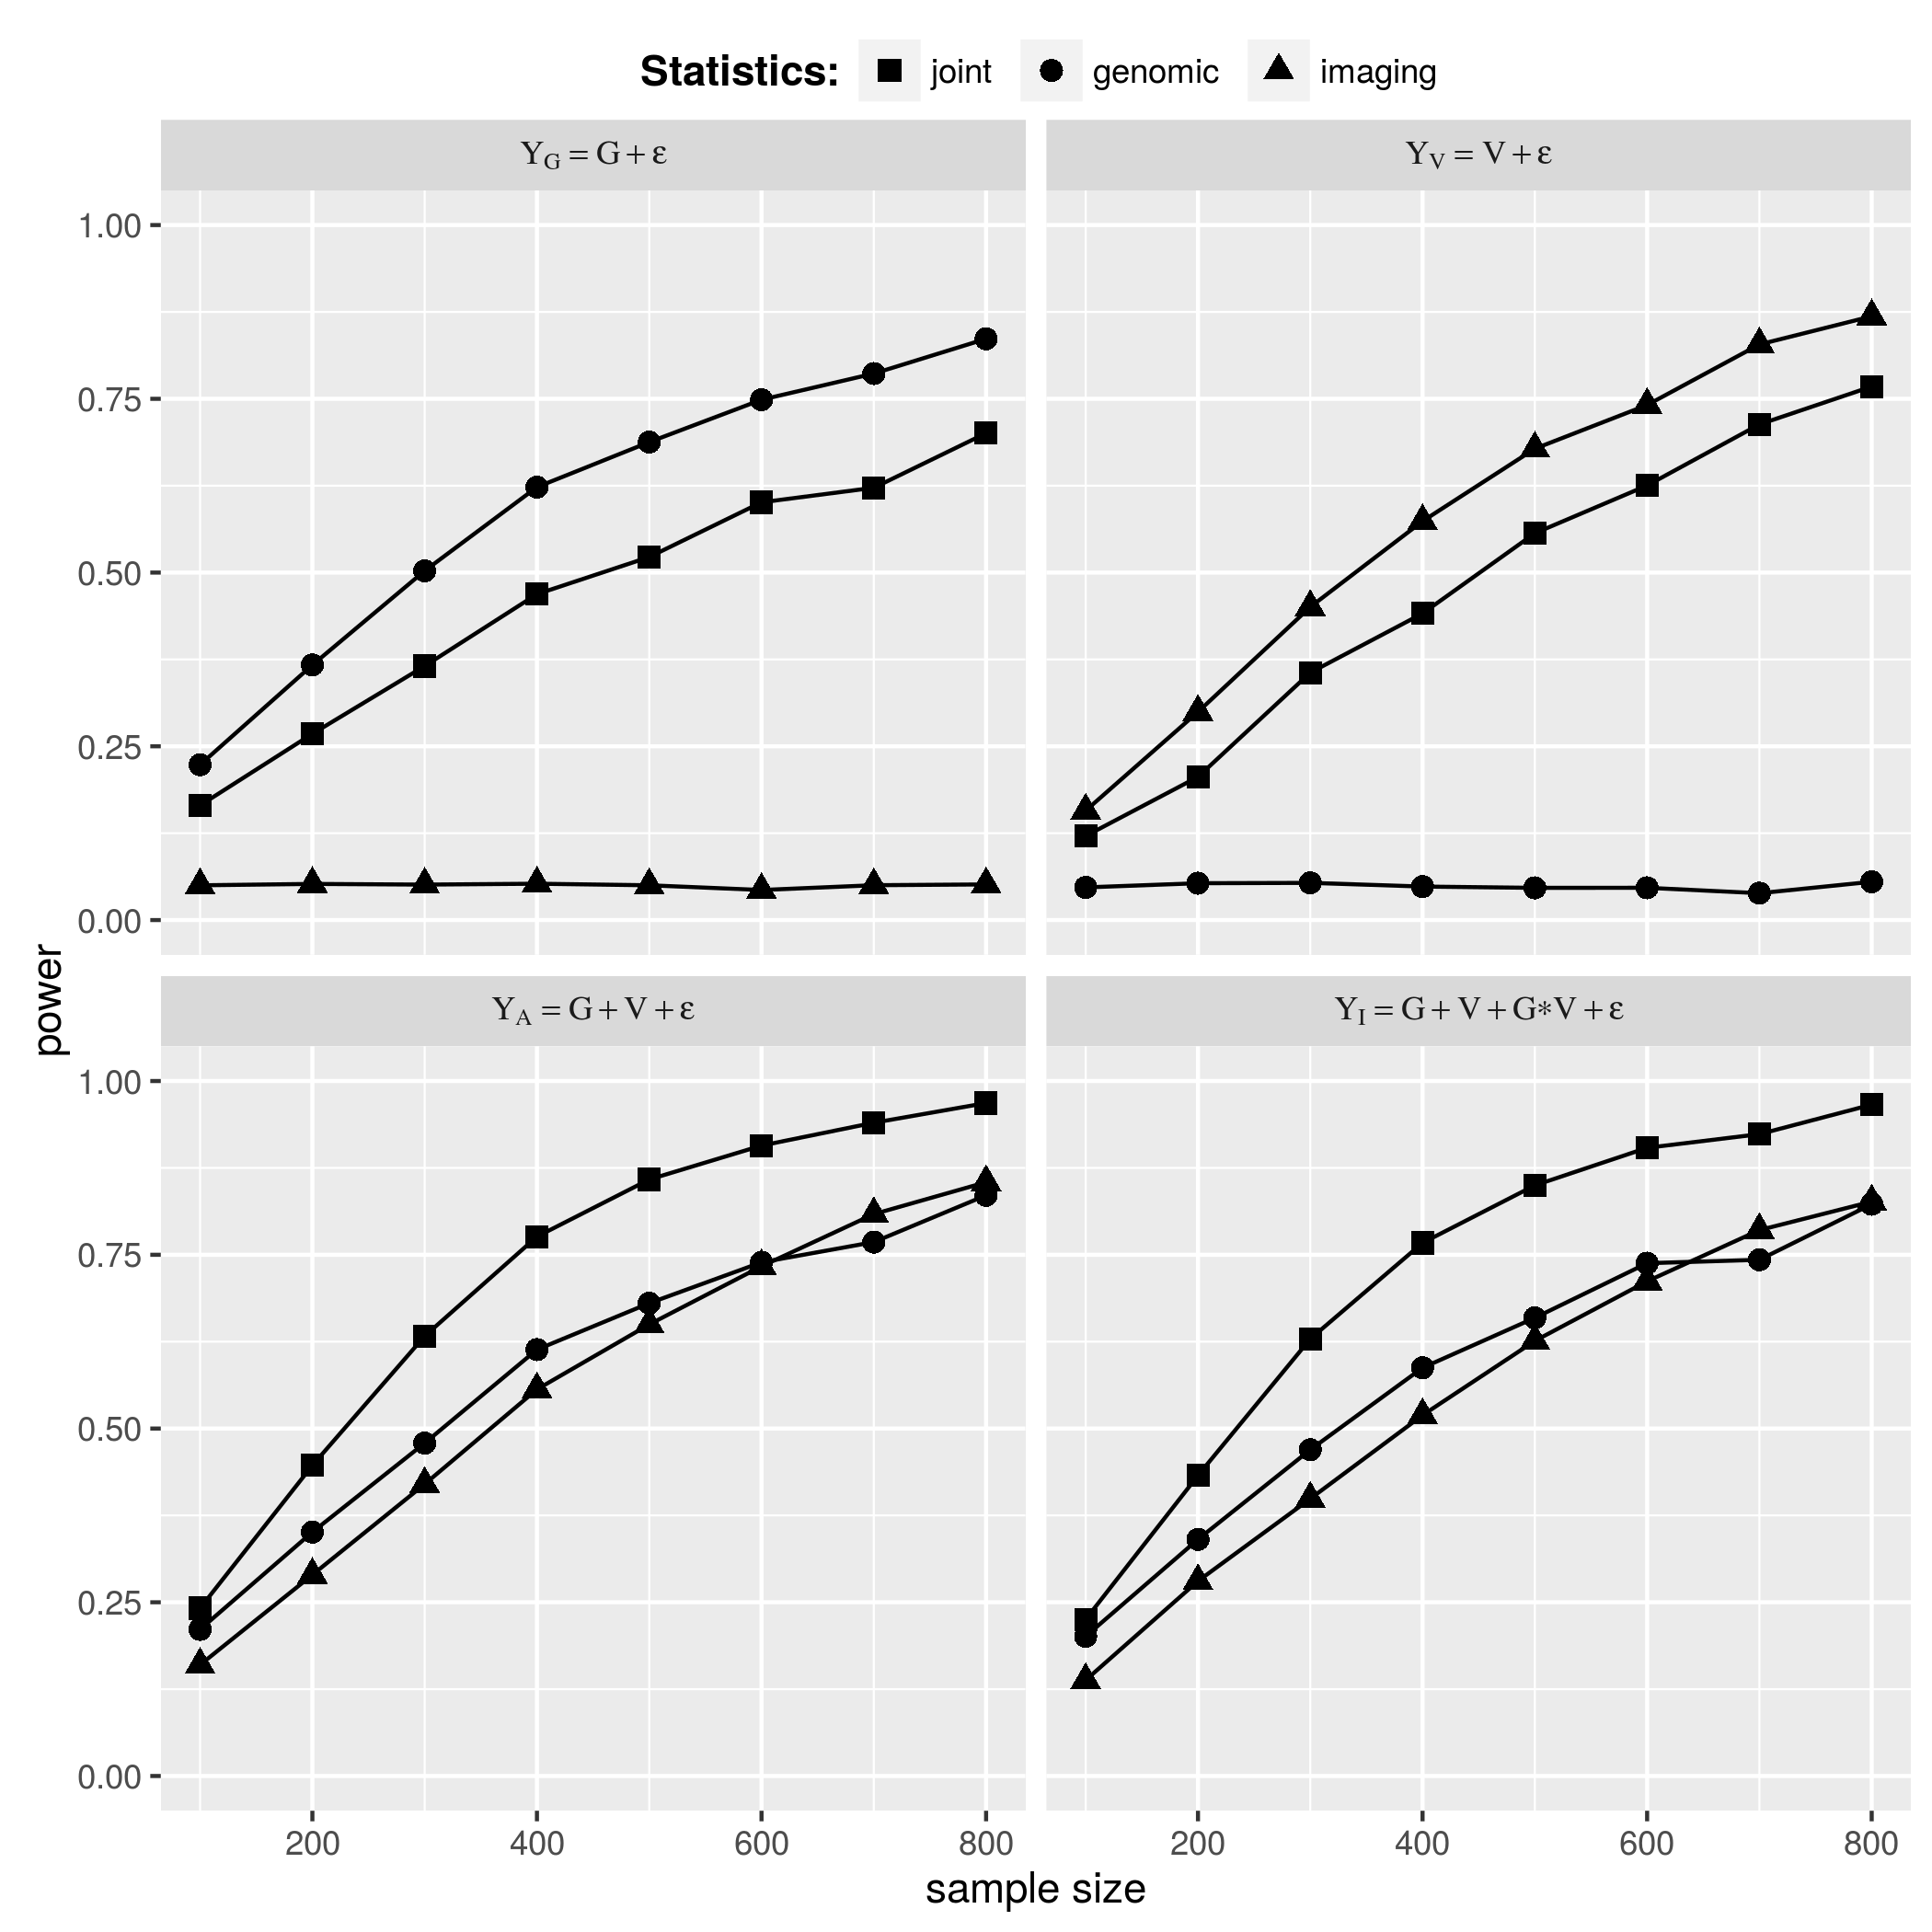
\includegraphics[width=400px]{img/PWR_CNT_KNL.png}
\caption{Joint U v.s. genetic U and imaing U}
\label{fig:PWR_CNT_KNL}
\end{figure}
The top row of Figure \ref{fig:PWR_CNT_KNL} shows the two simplified statistics $U_G$ and $U_V$ performed best when they are indeed parsimonious, that is, the underlying effects were also purely genomic or imaging based, respectively, but they are powerless when the actual effect composition does not concur the choice of kernel functions. In contrast, the joint statistic $U_J$ performed fairly close to the parsimonious models. The bottom row shows joint U outperformed others when the effect is additive or interactive.

\subsubsection{Grouping and Aggregation on Imaging}
Imaging variants do not suffer ``low MAF'' like rare genomic variants do, but grouping and aggregation technique may still be helpful by avoiding multiple testing. Under the same sample sizes and effect compositions, we evaluate the performance of cortex regional test versus false discovery rate (FDR) corrected VWA. Here we do not test $H_0^G$, since the test statistic $U_G$ does not rely on imaging profile. The result is shown in Figure \ref{fig:PWR_CNT_VWA}.
\begin{figure}[!htbp]
\centering
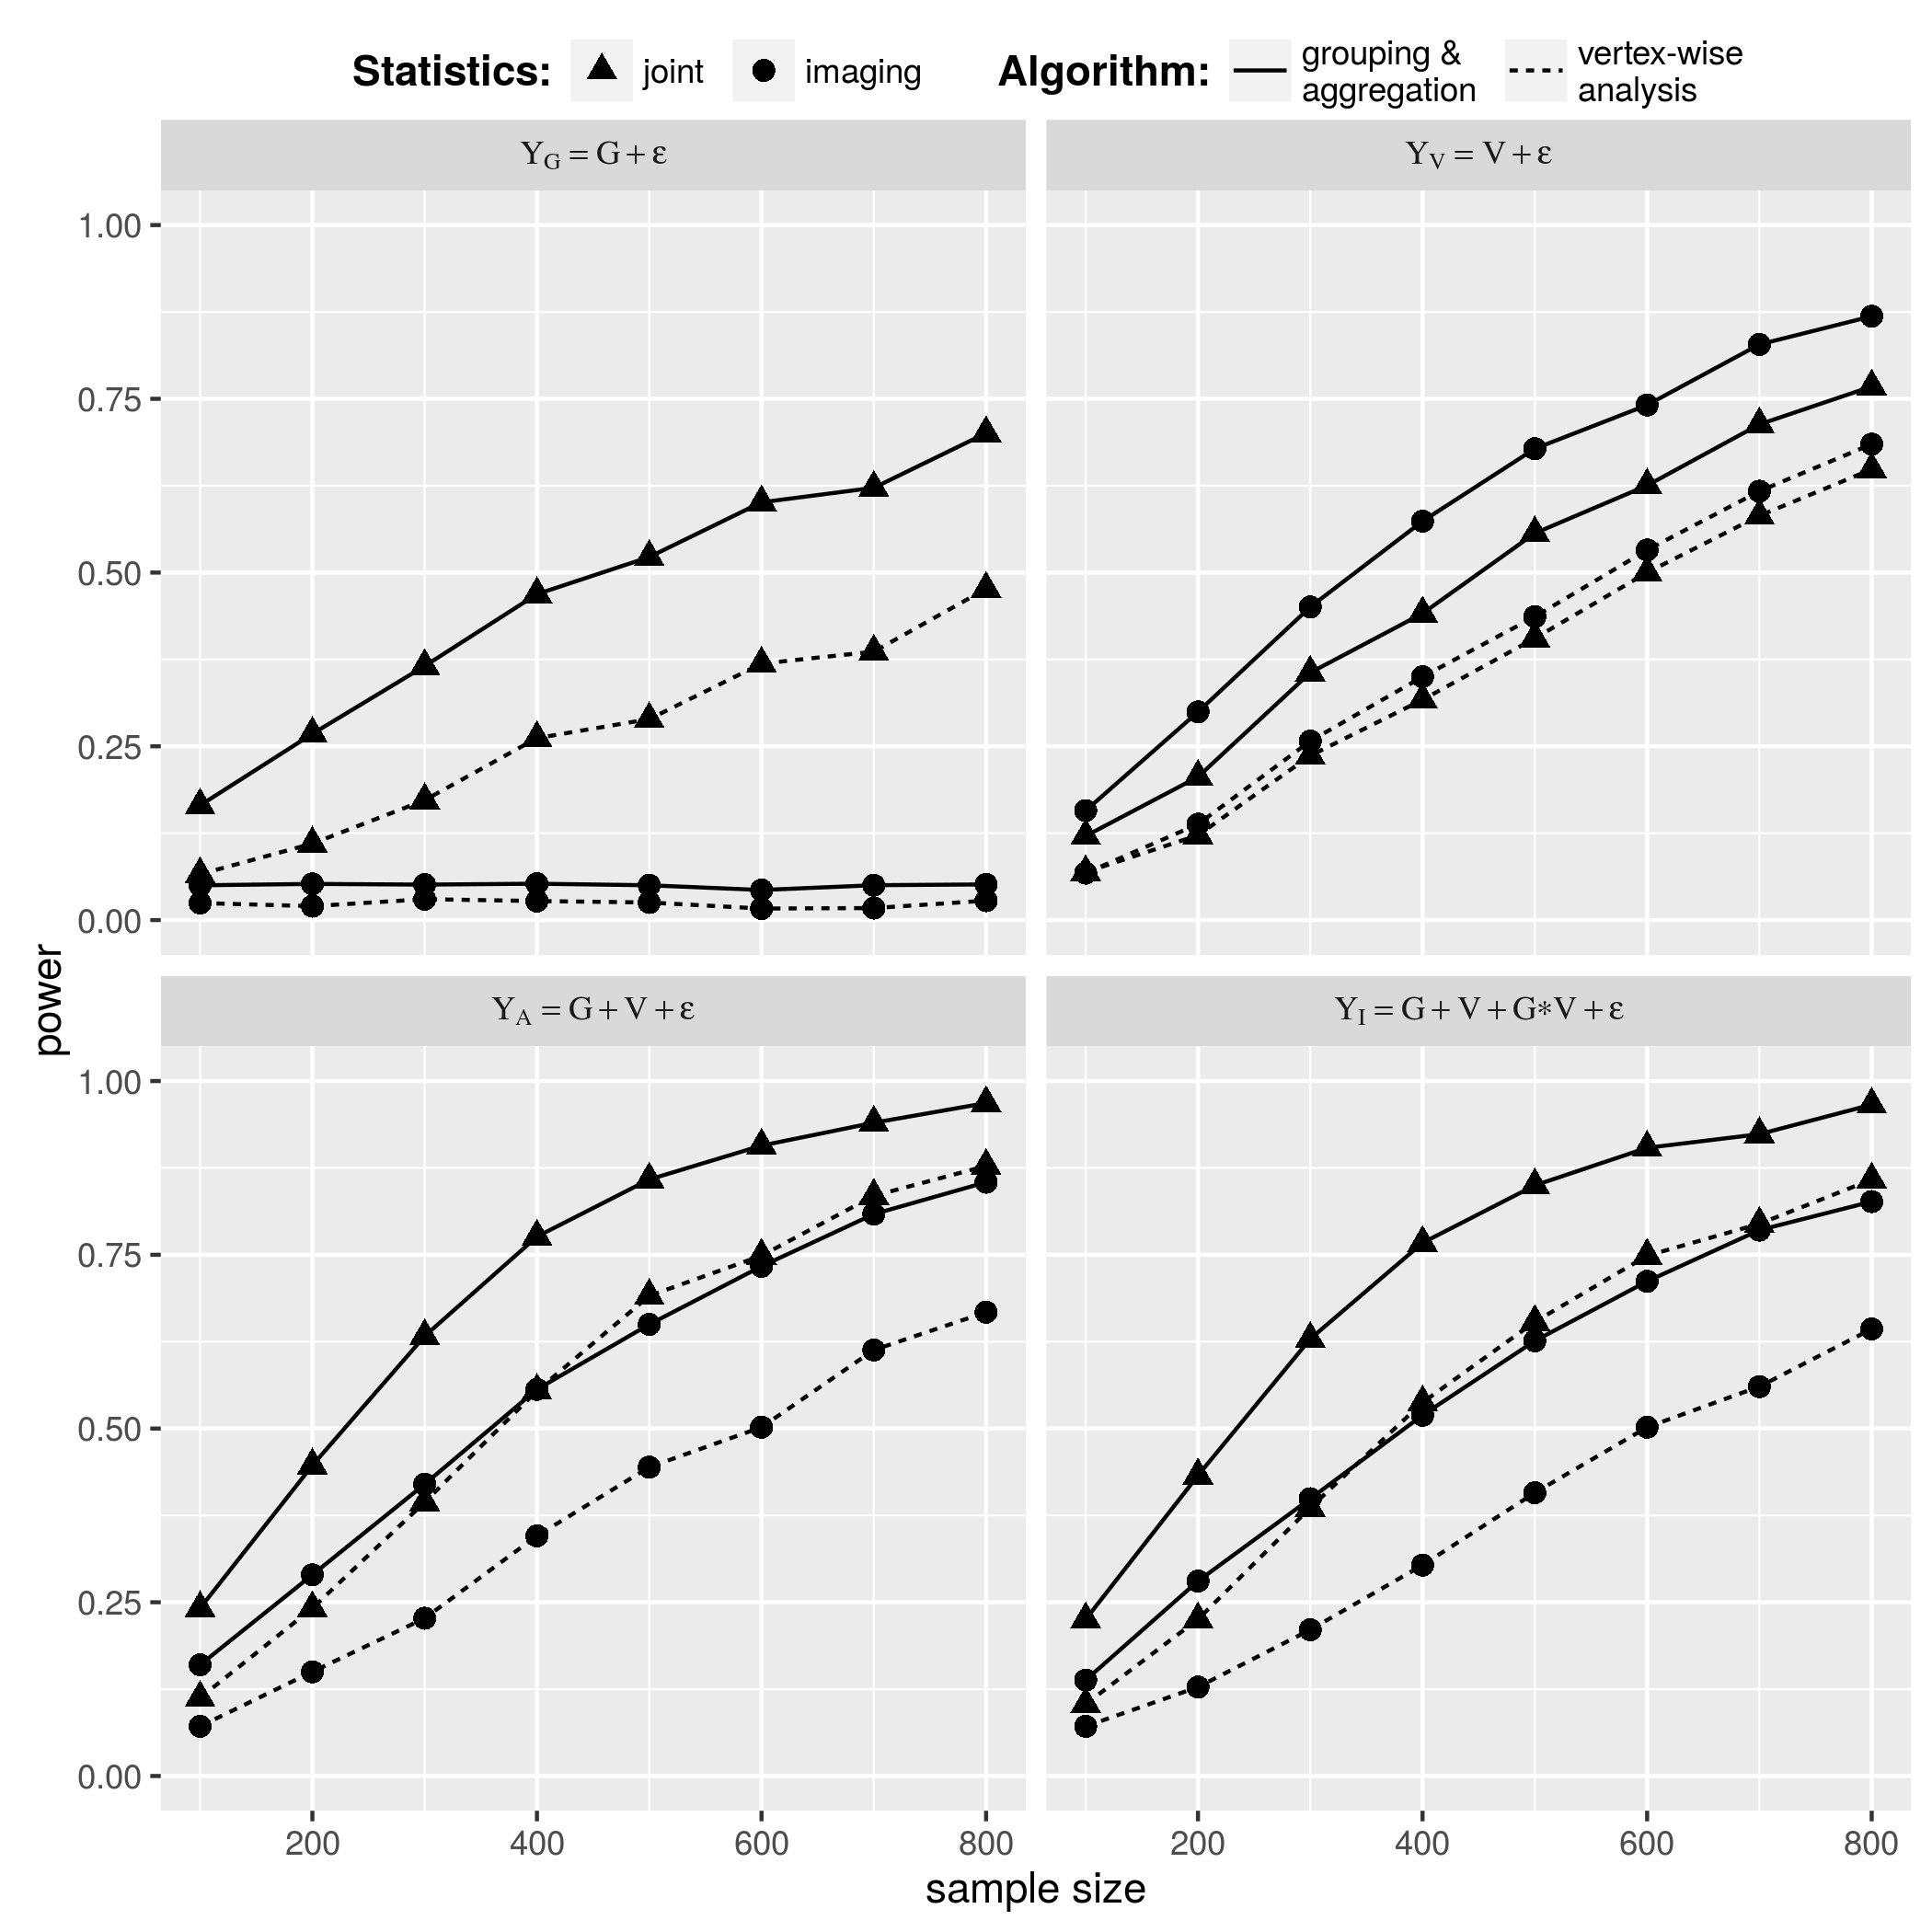
\includegraphics[width=400px]{img/PWR_CNT_VWA.png}
\caption{Grouping \& Aggregation v.s. Vertex-wise Analysis}
\label{fig:PWR_CNT_VWA}
\end{figure}
The aggregated test (solid lines) overpowers VWA (dashed lines) by a large margin in all scenarios. An interesting speculation happens when the U statistic is completely misspecified, the type I error rate of VWA is below 0.05 (Figure \ref{fig:PWR_CNT_VWA}, top left panel), which means the screening tests (512 of them) are highly correlated and caused FDR correction to be conservative. 

\subsubsection{Performance of High Order Imaging Features}
In this set of simulate we evaluation the use of high order features against the raw imaging profiles where they were abstracted from. Again tests of $H_0^G$ are opt out, the result is shown in Figure \ref{fig:PWR_CNT_SAE}.
\begin{figure}[!htbp]
\centering
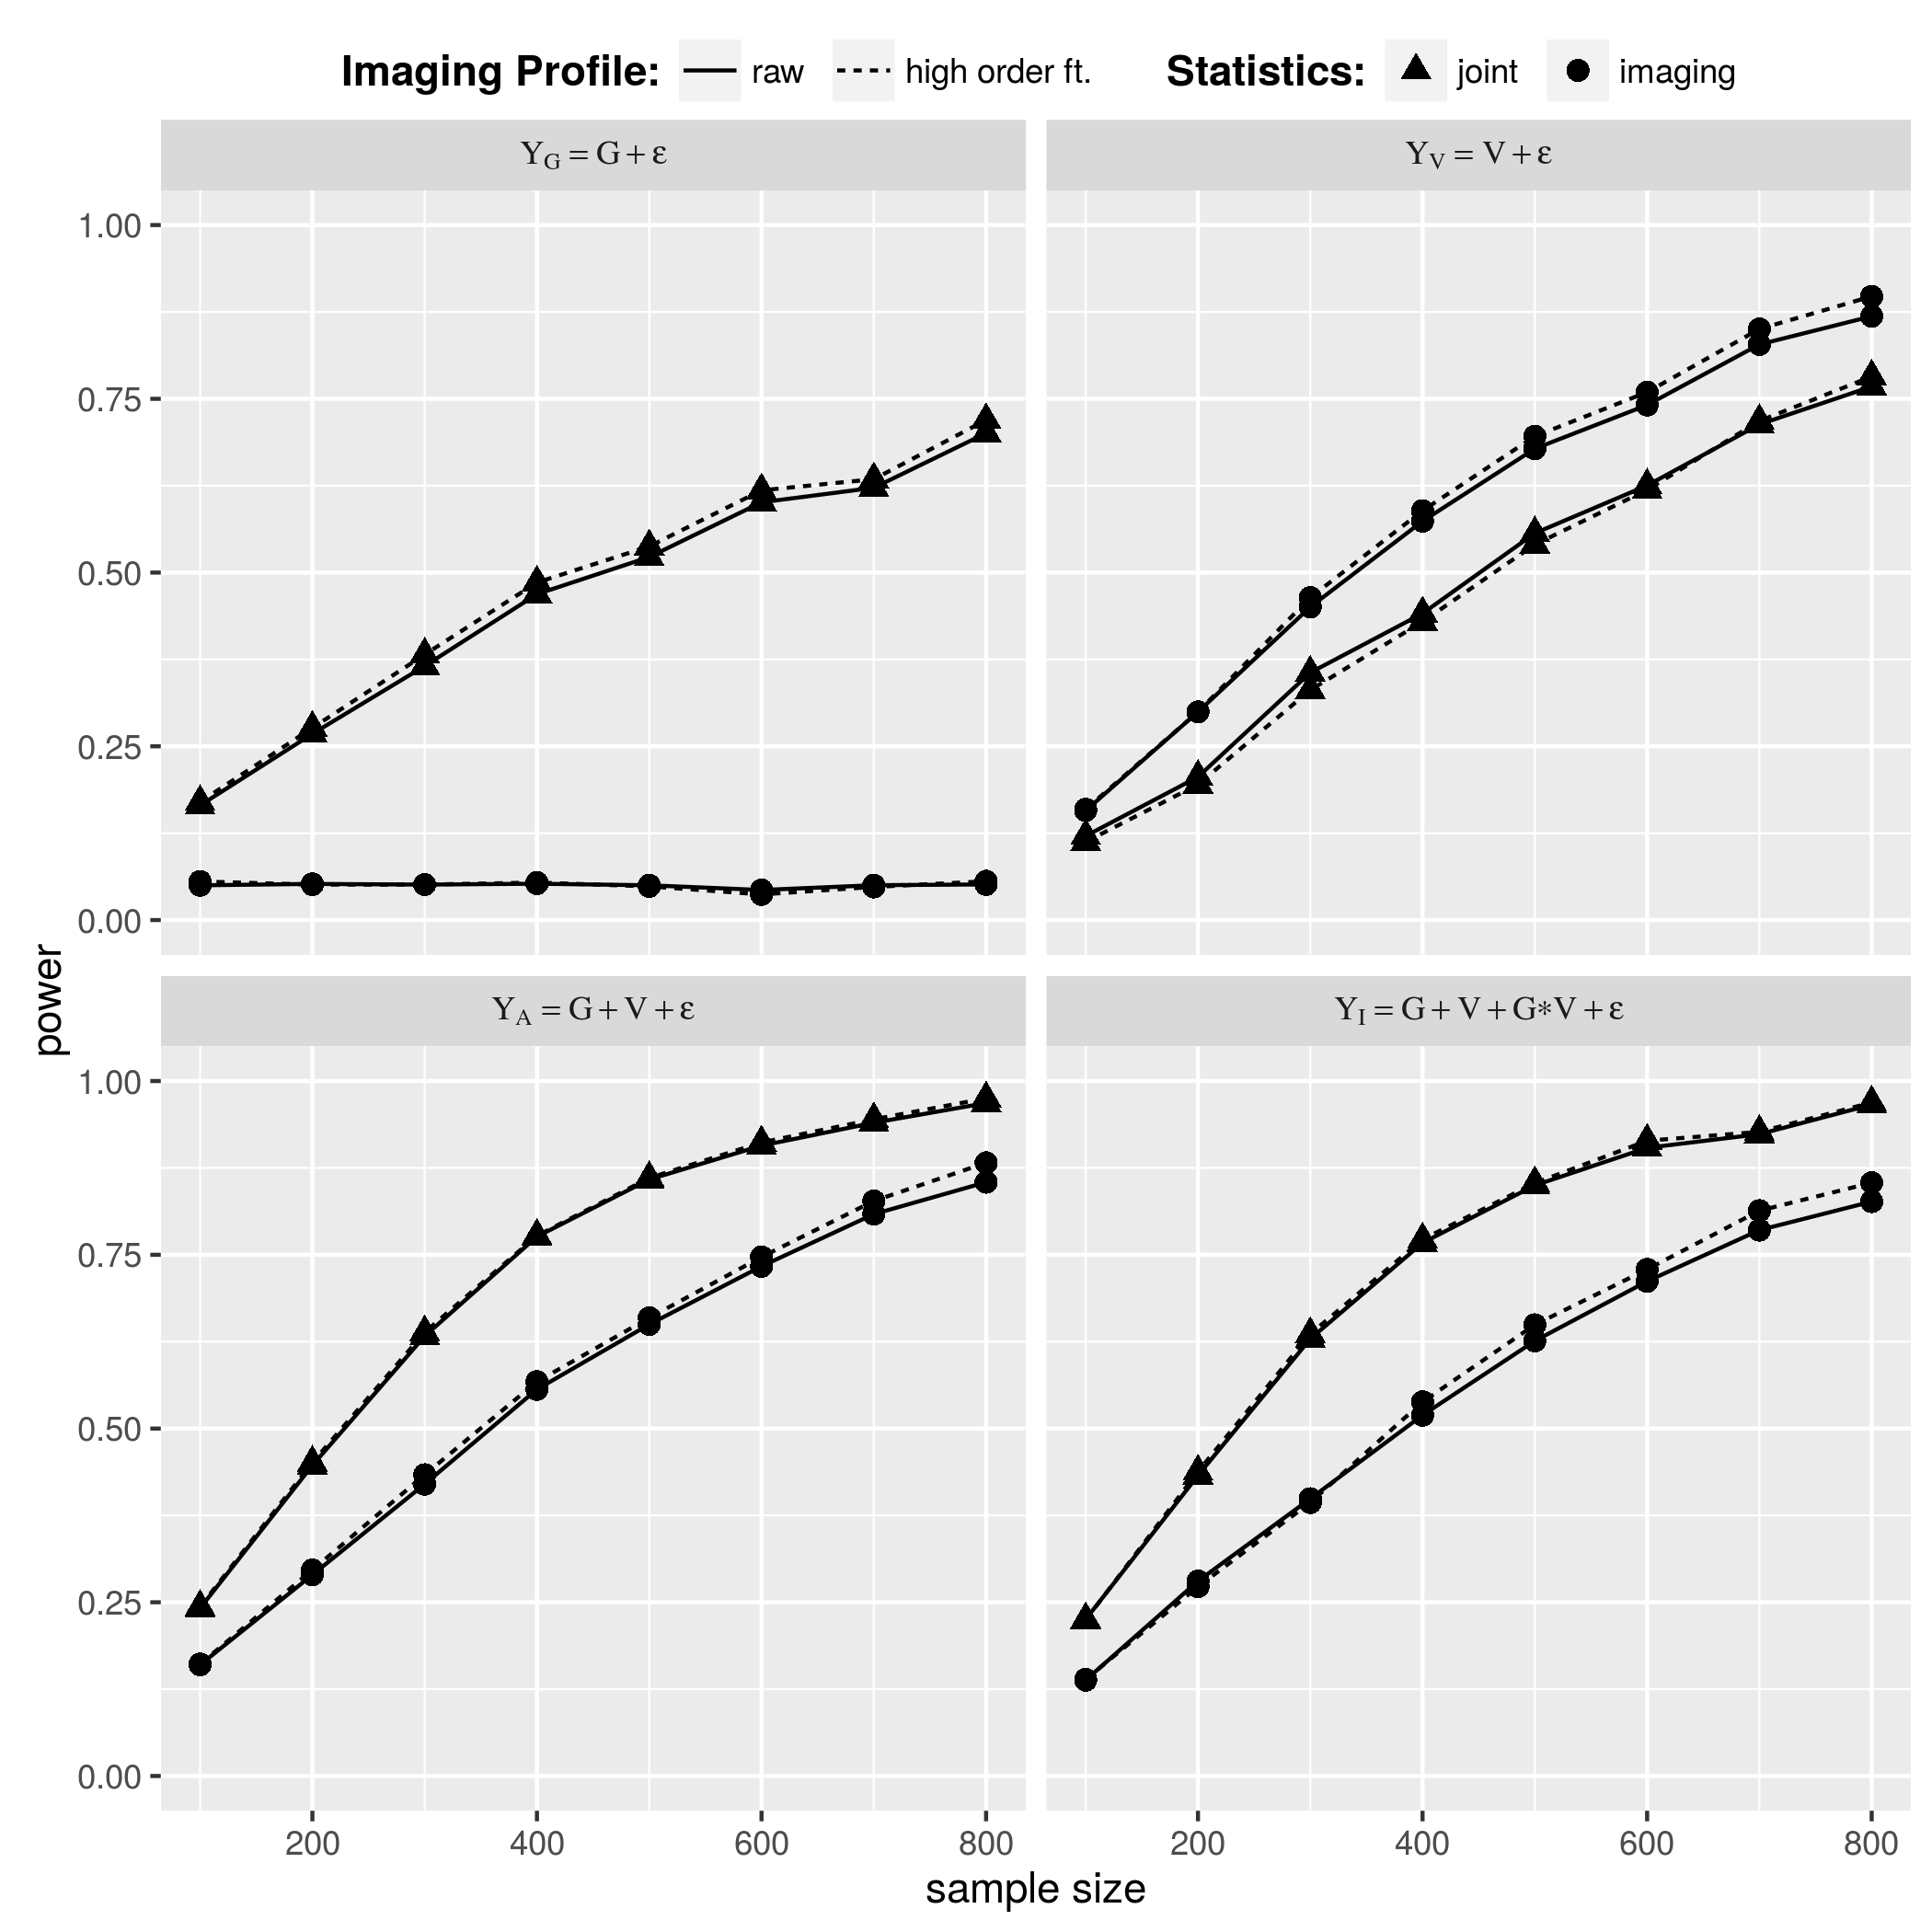
\includegraphics[width=400px]{img/PWR_CNT_SAE.png}
\caption{High Order Features v.s. Original Vertices}
\label{fig:PWR_CNT_SAE}
\end{figure}
Except the combination of lower sample size and the joint U statistic being partially misspecified (Figure \ref{fig:PWR_CNT_SAE}, top right), replacing raw imaging profile (Figure \ref{fig:PWR_CNT_SAE}, solid lines) with their high order features (Figure \ref{fig:PWR_CNT_SAE}, dashed lines) gains power, with the margin growing with the sample size. The top left panel in \ref{fig:PWR_CNT_SAE} also reassured that using high order features does not deviate the type I error rate.

\subsubsection{Binary phenotypes}
Four more dichotomous phenotypes are generated by sending the four continuous ones to inverse logit, then draw the case/control status from the resulting probabilities. In every scenario, the power performance shares very similar patterns to the report from continuous phenotype, shown in Figure \ref{fig:PWR_BIN_KNL}, \ref{fig:PWR_BIN_VWA} and \ref{fig:PWR_BIN_SAE}.

In general, the simulation studies demonstrated the capability of a joint test borrowing information from additional biomarkders (the imaging) to augment genetic association study, which is also robust when faced with uncertainty of the true composition of phenotype data generation process. Also demonstrated is the usefulness of grouping and aggregation strategy over alternative high dimensional profiles other than NGS, whose variants may not be ``rare'' but are correlated. Lastly, the high order features of low dimension outperforms their high dimensional raw imaging, not dramatically but getting better with larger samples.

\subsection{Real Data Analysis}
The baseline data of 327 out of 806 ADNI participants who has definite diagnosis status of Alzimer's Disease (AZ) entered the analysis, among whome 47 are cases and the rest 280 are healthy controls. The genomic testing units are $40,039$ gene regions. The imaging testing units are high order features of the 68 functional anatomy regions in the cortex, which is abstracted from the raw imaging by 68 corresponding SA trained with all 806 samples. We first regressed the the case/control status on 7 known risk factors of AD, namely age, gender, race, ethnicity, years of education, marriage status, ever smoking, and APOE $\epsilon$4 haplotype, then taken the residuals as the phenotype to construct U statistics. In total, there are $40,039 \times 68 = 2,722,652$ joint U statistic $U_J$ tested, for comparison, we also tested the two simplifed hypothesis $U_G$ and $U_V$ for every gene and cortex region, respective. Thus, the results came in triplets of p-values $P_G$, $P_V$ and $P_U$, corresponding to the three U statistics , and $U_J$. The triplets are show in Figure \ref{fig:RDA_PVL} horizontally, ordered by $P_J$, and for each triplets, the three p-values are lining up vertically by the negative log transformed value.
\begin{figure}[!htbp]
\centering
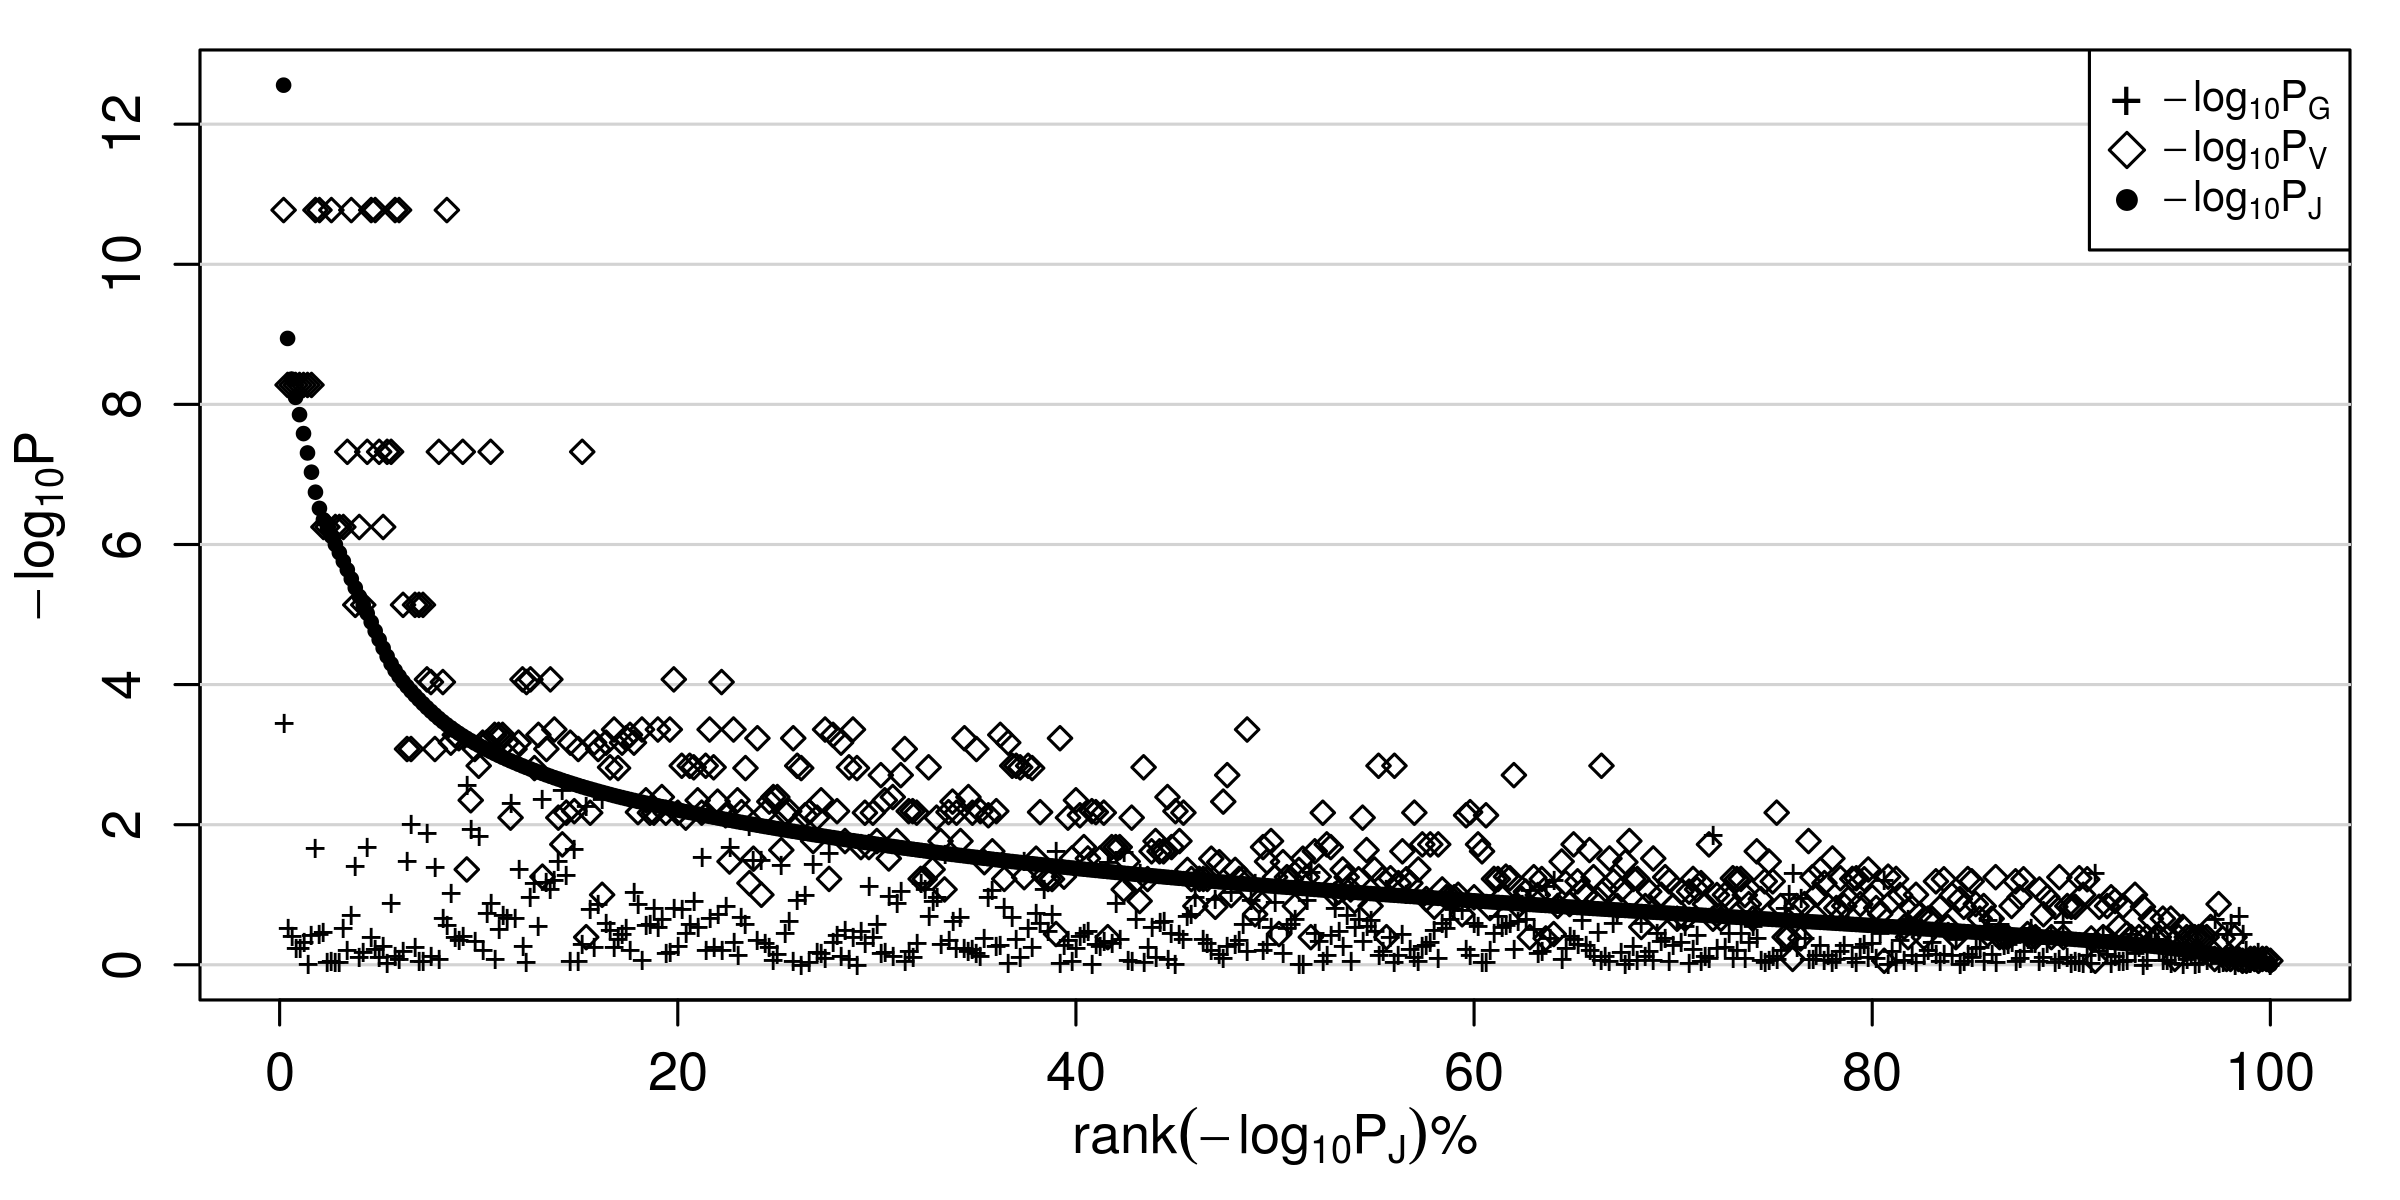
\includegraphics[width=\textwidth]{img/RDA_PVL.png}
\caption{p-values of real data analysis}
\label{fig:RDA_PVL}
\end{figure}
In general, the significance of the purely vertex based $U_G$ (Figure \ref{fig:RDA_PVL} diamonds) is above the purely genomic based $U_G$ (Figure \ref{fig:RDA_PVL} crosses), reflecting the fact that genomic effect is weak while the cortex profile is a very indicator of the diseases in brain, and the joint similarity U statistic $U_J$ (Figure \ref{fig:RDA_PVL} dots) lies between the two, leaning closer to the cortical vertex based $U_V$. To be noted is how $U_J$ ``borrow'' information from the cortex profile to enhance the statistical significance of the purely genomic based $U_G$, which by itself never reaches significance at the threshold of $0.05$ after the FDR adjustment of $40,039$ tests. When $U_G$ is also moderately significant, the corresponding joint statistic $U_J$ could be more significant than both $U_G$ and $U_V$, reaching the 0.05 threshold even after FDR adjustment over $2,680,894$ tests, which is shown by the dots in the most top left corner of Figure \ref{fig:RDA_PVL}, and reflected by the 20 top significant triplets listed in Table \ref{tab:RDA_T20}.
\begin{table}[!htbp]
\centering
\small
\caption{Top 20 most significant joint test - overall}
\label{tab:RDA_T20}
% latex table generated in R 3.3.1 by xtable 1.8-0 package
% Fri Dec 23 17:55:43 2016
\begin{tabular}{llcclll}
  \hline
  GENE & CORTEX & $|V|$ & $|G|$ & $\qquad P_G$ & \qquad $P_V$ & \qquad $P_J$ \\ 
  \hline
  IGLV1-44 & l.superiortemporal & 7271 &  174 & $3.51 \times {10^{-04}}$ & $1.68 \times {10^{-11}}{_+^*}$ & $2.77 \times {10^{-13}}{_+^*}$ \\ 
  NBEAP2 & l.superiortemporal & 7271 &  238 & $1.19 \times {10^{-04}}$ & $1.68 \times {10^{-11}}{_+^*}$ & $4.74 \times {10^{-13}}{_+^*}$ \\ 
  RPL21P89 & l.superiortemporal & 7271 &   90 & $6.36 \times {10^{-04}}$ & $1.68 \times {10^{-11}}{_+^*}$ & $5.14 \times {10^{-13}}{_+^*}$ \\ 
  LOC102724504 & l.superiortemporal & 7271 &   59 & $1.41 \times {10^{-03}}$ & $1.68 \times {10^{-11}}{_+^*}$ & $5.56 \times {10^{-13}}{_+^*}$ \\ 
  CNTNAP3P8 & l.superiortemporal & 7271 &   40 & $1.08 \times {10^{-03}}$ & $1.68 \times {10^{-11}}{_+^*}$ & $6.17 \times {10^{-13}}{_+^*}$ \\ 
  CDH4 & l.superiortemporal & 7271 & 9464 & $4.64 \times {10^{-03}}$ & $1.68 \times {10^{-11}}{_+^*}$ & $6.96 \times {10^{-13}}{_+^*}$ \\ 
  HNRNPA1P19 & l.superiortemporal & 7271 &   17 & $8.88 \times {10^{-04}}$ & $1.68 \times {10^{-11}}{_+^*}$ & $7.80 \times {10^{-13}}{_+^*}$ \\ 
  FAM72C & l.superiortemporal & 7271 &  174 & $9.28 \times {10^{-06}}$ & $1.68 \times {10^{-11}}{_+^*}$ & $7.82 \times {10^{-13}}{_+^*}$ \\ 
  RP11-638L3.1 & l.superiortemporal & 7271 & 4067 & $1.41 \times {10^{-1}}$ & $1.68 \times {10^{-11}}{_+^*}$ & $9.49 \times {10^{-13}}{_+^*}$ \\ 
  CPXM1 & l.superiortemporal & 7271 &  208 & $8.78 \times {10^{-4}}$ & $1.68 \times {10^{-11}}{_+^*}$ & $1.08 \times {10^{-12}}{_+^*}$ \\ 
  LOC101929612 & l.superiortemporal & 7271 &  256 & $1.44 \times {10^{-2}}$ & $1.68 \times {10^{-11}}{_+^*}$ & $1.15 \times {10^{-12}}{_+^*}$ \\ 
  LOC100996517 & l.superiortemporal & 7271 &   34 & $6.77 \times {10^{-4}}$ & $1.68 \times {10^{-11}}{_+^*}$ & $1.20 \times {10^{-12}}{_+^*}$ \\ 
  IGLV5-45 & l.superiortemporal & 7271 &  179 & $3.44 \times {10^{-4}}$ & $1.68 \times {10^{-11}}{_+^*}$ & $1.23 \times {10^{-12}}{_+^*}$ \\ 
  MIS18BP1 & l.superiortemporal & 7271 &  553 & $4.95 \times {10^{-3}}$ & $1.68 \times {10^{-11}}{_+^*}$ & $1.35 \times {10^{-12}}{_+^*}$ \\ 
  CDR2 & l.superiortemporal & 7271 &  260 & $1.82 \times {10^{-4}}$ & $1.68 \times {10^{-11}}{_+^*}$ & $1.39 \times {10^{-12}}{_+^*}$ \\ 
  RPL41P2 & l.superiortemporal & 7271 &   87 & $6.04 \times {10^{-3}}$ & $1.68 \times {10^{-11}}{_+^*}$ & $1.59 \times {10^{-12}}{_+^*}$ \\ 
  LOC101927737 & l.superiortemporal & 7271 &  157 & $7.20 \times {10^{-3}}$ & $1.68 \times {10^{-11}}{_+^*}$ & $1.60 \times {10^{-12}}{_+^*}$ \\ 
  IGLV1-47 & l.superiortemporal & 7271 &  138 & $1.44 \times {10^{-2}}$ & $1.68 \times {10^{-11}}{_+^*}$ & $1.60 \times {10^{-12}}{_+^*}$ \\ 
  IGLV7-46 & l.superiortemporal & 7271 &  130 & $9.15 \times {10^{-4}}$ & $1.68 \times {10^{-11}}{_+^*}$ & $1.69 \times {10^{-12}}{_+^*}$ \\ 
  ZDHHC15 & l.superiortemporal & 7271 &   80 & $1.56 \times {10^{-3}}$ & $1.68 \times {10^{-11}}{_+^*}$ & $1.73 \times {10^{-12}}{_+^*}$ \\ 
  \hline
  \multicolumn{7}{l}{\texttt{*: below 0.05 after Bonferroni correction}} \\ 

  \multicolumn{7}{l}{\texttt{+: below 0.01 after FDR correction}}        \\ \hline
\end{tabular}
 \\
\texttt{*: below 0.05 after Bonferroni correction} \\
\texttt{+: below 0.05 after FDR correction}
\end{table}
From Table \ref{tab:RDA_T20} we see the top 20 most significant test all involves the left superior temporal cortex, whose neuron loss and shrinkage in volume is highly associated with the onset of Alzheimer's Disease and its progression to dementia \cite{AD:ST1}. 

To see some more diverse cases of cortex profile ``lending'' information to the genomic test to enhance the significance of joint statistic $U_J$, we compiled the most significant $U_J$ involving each of the 68 regions, and listed the top 20 in Table \ref{tab:RDA_JNT}.
\begin{table}[!htbp]
\centering
\small
\caption{top 20 most significant joint test - per cortical region}
\label{tab:RDA_JNT}
% latex table generated in R 3.3.1 by xtable 1.8-0 package
% Fri Dec 23 17:55:45 2016
\begin{tabular}{llcclll}
  \hline
GENE & CORTEX & $|V|$ & $|G|$ & $\qquad P_G$ & \qquad $P_V$ & \qquad $P_J$ \\ 
  \hline
IGLV1-44 & l.superiortemporal & 7271 &  174 & $3.51 \times {10^{-4}}$ & $1.68 \times {10^{-11}}{_+^*}$ & $2.77 \times {10^{-13}}{_+^*}$ \\ 
  ZNF749 & l.entorhinal & 1102 &  321 & $2.67 \times {10^{-5}}$ & $5.28 \times {10^{-9}}{_+^*}$ & $2.63 \times {10^{-11}}{_+^*}$ \\ 
  FAM72C & r.superiortemporal & 6868 &  174 & $9.28 \times {10^{-6}}$ & $4.75 \times {10^{-8}}{_+^*}$ & $2.14 \times {10^{-10}}{_+^*}$ \\ 
  ZNF749 & r.entorhinal &  902 &  321 & $2.67 \times {10^{-5}}$ & $5.62 \times {10^{-7}}{_+^*}$ & $1.08 \times {10^{-9}}{_+^*}$ \\ 
  FAM72C & l.cuneus & 1630 &  174 & $9.28 \times {10^{-6}}$ & $7.27 \times {10^{-6}}{_+^*}$ & $4.22 \times {10^{-9}}{_+^*}$ \\ 
  ZNF749 & l.fusiform & 4714 &  321 & $2.67 \times {10^{-5}}$ & $8.43 \times {10^{-5}}{_+^*}$ & $4.54 \times {10^{-8}}{_+}$ \\ 
  FAM72C & l.middletemporal & 4452 &  174 & $9.28 \times {10^{-6}}$ & $4.38 \times {10^{-4}}{_+^*}$ & $5.14 \times {10^{-8}}{_+}$ \\ 
  FAM72C & r.cuneus & 1638 &  174 & $9.28 \times {10^{-6}}$ & $8.31 \times {10^{-4}}{_+}$ & $6.33 \times {10^{-8}}{_+}$ \\ 
  ZNF749 & l.temporalpole &  839 &  321 & $2.67 \times {10^{-5}}$ & $9.20 \times {10^{-5}}{_+^*}$ & $7.05 \times {10^{-8}}{_+}$ \\ 
  FAM72C & r.precuneus & 7975 &  174 & $9.28 \times {10^{-6}}$ & $1.44 \times {10^{-3}}{_+}$ & $7.43 \times {10^{-8}}{_+}$ \\ 
  HSPD1P13 & l.pericalcarine & 1912 &   86 & $1.69 \times {10^{-5}}$ & $6.74 \times {10^{-4}}{_+^*}$ & $1.12 \times {10^{-7}}{_+}$ \\ 
  FAM72C & r.fusiform & 4661 &  174 & $9.28 \times {10^{-6}}$ & $5.83 \times {10^{-4}}{_+^*}$ & $1.18 \times {10^{-7}}{_+}$ \\ 
  HSPD1P13 & r.pericalcarine & 1823 &   86 & $1.69 \times {10^{-5}}$ & $5.22 \times {10^{-4}}{_+^*}$ & $1.50 \times {10^{-7}}{_+}$ \\ 
  FAM72C & r.precentral & 10705 &  174 & $9.28 \times {10^{-6}}$ & $6.73 \times {10^{-3}}$ & $2.15 \times {10^{-7}}{_+}$ \\ 
  HSPD1P13 & r.paracentral & 3831 &   86 & $1.69 \times {10^{-5}}$ & $1.91 \times {10^{-2}}$ & $2.41 \times {10^{-7}}{_+}$ \\ 
  ZNF749 & r.temporalpole &  817 &  321 & $2.67 \times {10^{-5}}$ & $1.55 \times {10^{-3}}{_+}$ & $3.30 \times {10^{-7}}{_+}$ \\ 
  FAM72C & l.precentral & 10740 &  174 & $9.28 \times {10^{-6}}$ & $6.62 \times {10^{-3}}$ & $3.94 \times {10^{-7}}{_+}$ \\ 
  FAM72C & l.superiorfrontal & 12179 &  174 & $9.28 \times {10^{-6}}$ & $1.96 \times {10^{-3}}{_+}$ & $4.39 \times {10^{-7}}{_+}$ \\ 
  FAM72C & l.postcentral & 9519 &  174 & $9.28 \times {10^{-6}}$ & $1.71 \times {10^{-2}}$ & $5.69 \times {10^{-7}}{_+}$ \\ 
  ZNF749 & l.insula & 5229 &  321 & $2.67 \times {10^{-5}}$ & $1.52 \times {10^{-3}}{_+}$ & $6.69 \times {10^{-7}}{_+}$ \\ 
   \hline
    \multicolumn{7}{l}{\texttt{*: below 0.05 after Bonferroni correction}} \\ 

    \multicolumn{7}{l}{\texttt{+: below 0.01 after FDR correction}}        \\ \hline
\end{tabular}
 \\
\texttt{*: below 0.05 after Bonferroni correction} \\
\texttt{+: below 0.05 after FDR correction}
\end{table}
We see in some cases both the genome and cortex based $U_G$ and $U_V$ do not reach statistical significance after multiple testing adjustment yet the joint statistic $U_J$ does, even if the number of tests ($2,680,894$) is way larger than the number of genes ($40,039$) or cortical regions ($68$). These result suggest the existence of strong interaction of unknown type between the corresponding gene and cortex. Because the test is backed by grouping and signal aggregation, also the abstracted features which is 16 times smaller than the original cortex are used, the entire analysis of $2,680,894$ triplets can be quickly done in 12 hours in the MSU HPCC clusters.